\PassOptionsToPackage{force}{filehook}

\documentclass{beamer}
\usecolortheme{wolverine}
\setbeamersize{text margin left=5mm,text margin right=5mm}
\setbeamertemplate{footline}[frame number]
\usepackage[normalem]{ulem}
%\useoutertheme{split}
%\useinnertheme{rounded}
\usepackage{pgf,tikz}
\usetikzlibrary{positioning}
\usepackage{amsmath}
\usepackage{enumitem}
\usepackage{amsfonts}
\usepackage{graphicx} 
\usepackage{subcaption}
\usepackage{hyperref}
\usepackage{cancel}
\usepackage{wrapfig}
\usepackage{comment}
\hypersetup{
	colorlinks=true,
	linkcolor=blue,
	filecolor=magenta,      
	urlcolor=cyan,
}
\usepackage{color}
\usepackage{mathpazo}
\usepackage{hyperref}
\usepackage{multimedia}
\usepackage{graphicx}
%\usepackage[demo]{graphicx}
\usepackage{caption}
\usepackage{subcaption}
%\usepackage{textcomp}
\usepackage{graphicx} 
\usepackage{booktabs}
\usepackage{cite}
\usepackage{hyperref}
\usepackage{multicol}
\usepackage{multirow,array}
\renewcommand{\arraystretch}{1.5}
\usepackage{amsmath}
\usepackage{mathrsfs}
\usepackage{amssymb}
\usepackage[utf8]{inputenc}
\usepackage{amsthm}
\newtheorem{thm}{Teorema}
\newtheorem{lem}[thm]{Lema}
\newtheorem{axiom}[thm]{Axioma}
\newtheorem{prop}[thm]{Proposici\'on}
\newtheorem{cor}[thm]{Corolario}
\theoremstyle{definition}
\newtheorem{defn}{Definici\'on}
\DeclareGraphicsExtensions{.pdf,.jpeg,.png,.eps}
%\usetheme{CambridgeUS}
\setbeamertemplate{navigation symbols}{}
\usepackage{pgf,tikz}
\usetikzlibrary{positioning}
\usepackage[spanish, activeacute]{babel} %Definir idioma español
\usepackage[utf8]{inputenc} %Codificacion utf-8
\usepackage{multirow}
\def\mydate{\leavevmode\hbox{\twodigits\day/\twodigits\month/\the\year}}
\def\twodigits#1{\ifnum#1<10 0\fi\the#1}

\def\mydate{\leavevmode\hbox{\twodigits\day/\twodigits\month/\the\year}}
\def\twodigits#1{\ifnum#1<10 0\fi\the#1}
\definecolor{rosee}{rgb}{0.7,0.05,0.25}
\usepackage[final]{pdfpages}

\title{Microeconom\'ia}
\subtitle{Maximizaci\'on de Beneficios \\ \mydate}
\author[Maximización de beneficios]{Lara Sánchez Peña\footnote{Basado en las notas de Marcos Ariel Lissauer}}
\institute[]{UTDT}
\medskip
\date[UTDT 2023]{}

%   Esconder las soluciones
\newif\ifhideproofs
\hideproofstrue %uncomment to hide proofs

\ifhideproofs
\usepackage{environ}
\NewEnviron{hide}{}
\let\solucion\hide
\let\endsolucion\endhide
\fi
% - Either use conference name or its abbreviation.
% - Not really informative to the audience, more for people (including
%   yourself) who are reading the slides online

%\subject{}}
% This is only inserted into the PDF information catalog. Can be left
% out. 

% If you have a file called "university-logo-filename.xxx", where xxx
% is a graphic format that can be processed by latex or pdflatex,
% resp., then you can add a logo as follows:

% \pgfdeclareimage[height=0.5cm]{university-logo}{university-logo-filename}
% \logo{\pgfuseimage{university-logo}}

% Delete this, if you do not want the table of contents to pop up at
% the beginning of each subsection:
%\AtBeginSubsection[]
%{
  %\begin{frame}<beamer>{Outline}
    %\tableofcontents[currentsection,currentsubsection]
  %\end{frame}
%}

% Let's get started
\begin{document}
\begin{frame}
  \titlepage
\end{frame}

\begin{frame}{Objetivos}

\begin{itemize}
    \item ¿Cómo modelamos el comportamiento de las firmas?
    \item ¿Qué decisiones puede tomar una firma?
    \item ¿Cómo se diferencia el problema de la firma en el corto y en el largo plazo? ¿Cómo se maximizan beneficios en el corto/ largo plazo?
      \item ¿Qué propiedades de la tecnología son necesarias para garantizar que los beneficios se maximizan?
      \item Veremos cómo obtener las demandas no condicionadas de insumos $x_i^*$ ($i=1,2$), cuál es la función de oferta de bien final y estudiaremos sus propiedades.
      \item ¿Cómo cambia el beneficio máximo si aumenta en el \textbf{margen} $p$? ¿Cómo cambia el beneficio máximo si aumenta en el \textbf{margen} $w_1$? \textbf{Lema de Hotelling.}
    \item Si la firma usa una tecnología con \textbf{rendimientos constantes a escala}, en un mercado \textbf{perfectamente competitivo}, los beneficios \textbf{en equilibrio} son iguales a 0.
    \item Material de repaso: Ver las slides de Eco 1 en el campus 6.1.
\end{itemize}
\end{frame}

\begin{frame}{Comportamiento y decisiones de la firma}
    El objetivo para la firma es la \textbf{maximizar el beneficio}.

    La firma puede decidir:
    \begin{itemize}
        \item \textbf{No producir}. En el \textbf{corto plazo} la firma paga los \textbf{costos fijos} y en el \textbf{largo plazo} la firma \textbf{sale del mercado y no paga nada}.
        \item \textbf{Producir}.
        \begin{itemize}
            \item Cuánto comprar de los insumos disponibles. En el \textbf{corto plazo} puede elegir cuánto comprar del insumo 1, $x_1$. En el \textbf{largo plazo} puede elegir cuánto comprar de los insumos 1 y 2, $(x_1,x_2)$.
            \item Cuánto vender del bien que produce $y$.
            \item \sout{A qué precio vende el bien, teniendo en cuenta la demanda.}\footnote{Si la firma fuera \textbf{no competitiva} podría elegir el precio al que vende, pero por gran parte de la materia supondremos que las firmas \textbf{sí son competitivas}.} 
        \end{itemize}
    \end{itemize}
\end{frame}




%\begin{frame}{Los beneficios}
%\begin{itemize}
%\item Los beneficios se definen como los ingresos menos los costos. Supongamos que la firma produce $n$ bienes $(y_1,…,y_n)$ y utiliza $m$ factores $(x_1,…, x_m)$. Sean $(p_1,…, p_n)$ los precios de los productos y $(w_1,…, w_n)$ los precios de los factores. Los beneficios que obtiene la firma, $\pi$, pueden expresarse de la forma siguiente:
%\begin{center}
%$\pi=\color{blue}\sum\limits_{i=1}^np_iy_i\color{red}-\sum\limits_{i=1}^{m}w_{i}x_{i}$
%\end{center}
%\color{black}
%\item El primer término es el \color{blue}ingreso total \color{black} y el segundo el \color{red}costo total\color{black}.
%\end{itemize}
%\end{frame}
%\begin{frame}{Costos}
%\begin{itemize}
%\item Los costos económicos $w_i$ se miden en \$ y se miden como \textbf{costo de oportunidad}. Esto quiere decir que $w_i$ va a valer según el beneficio que obtendríamos según la alternativa más rentable (aparte de lo que estemos haciendo).

%Por ejemplo, el insumo $1$ es chocolate y puede ser usado para hacer barras de chocolate o bombones. Si por cada unidad de insumo de chocolate podemos ganar \$7 en barras de chocolate o \$4 con bombones, entonces la firma elegirá producir barras de chocolate y  $w_1=4$.

%\item Notar que como todas las firmas puede elegir entre las mismas alternativas, los costos $w_i$ son los mismos para todas.


%Por ejemplo, cuando una firma tiene dos oportunidades de inversión, A y B, el costo de oportunidad de elegir el proyecto A es el beneficio del proyecto B.

%El término se basa en la idea de que si un individuo utiliza, por ejemplo, su trabajo, pierde la oportunidad de emplearlo en otra parte. Por lo tanto, los salarios perdidos forman parte del costo de producción.
%\item La \textbf{definición económica del beneficio} implica valorar todos los factores y los productos a su \textbf{costo de oportunidad}. 

%\item Los \textbf{contadores}, a la hora de calcular costos $w_i$, utilizan los costos históricos (es decir, lo que costó el factor cuando se compró). Por otro lado, los \textbf{economistas} toman en cuenta los costos de oportunidad.
%Tal como lo calculan los contadores, no mide necesariamente con precisión los beneficios económicos, ya que normalmente éstos utilizan los costos históricos (es decir, lo que costó el factor cuando se compró) en lugar de los costos económicos (es decir, lo que costaría si se comprara hoy). El término ``beneficio'' se utiliza en sentidos muy distintos, pero nosotros siempre nos atendremos a la definición económica.
%\end{itemize}
%\end{frame}

%\begin{frame}{Los Beneficios}
%\begin{itemize}
%\item Normalmente, suponemos que los factores son \textit{variables flujo}. Un número dado de horas semanales y un número dado de horas-máquina semanales generan una determinada cantidad de producción a la semana. En ese caso, los precios de los factores son los que corresponden a la adquisición de dichos flujos. Los salarios se expresan, lógicamente, en pesos por hora. En el caso de las máquinas, la medida análoga es el alquiler, es decir, la tasa a la que podemos alquilar una máquina durante el periodo de tiempo dado.
%\item Muchas veces, no existe un mercado muy desarrollado de máquinas de alquiler, ya que las firmas suelen comprar su equipo de capital. En estos casos tenemos que obtener el alquiler implícito calculando cuánto costaría comprar una máquina al principio del periodo y venderla al final.
%\end{itemize}
%\end{frame}




\begin{frame}{Maximización del beneficio en el corto plazo}
\begin{itemize}
	\item Consideremos una firma que produce un \textbf{un bien final} utilizando \textbf{dos insumos}.\footnote{A los \textbf{insumos} también se los llama \textbf{factores de producción}.}
	\item En el \textbf{corto plazo}, el insumo 2 est\'a fijo en un valor $x_{2}=k$.
	\item El problema de la firma se resume en:
	\begin{equation*}\hspace{-3em}
	\max_{x_{1},y}py-w_{1}x_{1}-w_{2}k\quad s.a. \quad (1)\, y\leq f(x_{1},k) ; \, (2) \,y\geq 0;\, (3) \,x_{1}\geq 0 
	\end{equation*}
 %	\item Recordemos que según nuestros supuestos, \textbf{todos los planes eficientes están sobre la frontera} del conjunto de producción. Es decir, cuando $y= f(x_{1},k)$.
	\item Para maximizar los beneficios, se produce con $y=f(x_1,k)$.
	\begin{equation*}
	\max_{x_{1}}pf(x_{1},k)-w_{1}x_{1}-w_{2}k
	\end{equation*}

 
	\end{itemize}
\end{frame}

\begin{frame}{¿Cómo se resuelve la maximización de beneficios?}
    \textbf{Dependiendo de la tecnología}, resolveremos el problema de maximización de beneficios:
	\begin{enumerate}
	    \item derivando y obteniendo condición(es) de primer orden
	    \item analizando caso por caso (\underline{por ejemplo:} sustitutos perfectos, complementarios perfectos)
	\end{enumerate}

\medskip

\textbf{Nota importante:} Los costos unitarios $w_i$ se miden en \$ y se miden como \textbf{costo de oportunidad}. Como todas las firmas puede elegir entre las mismas alternativas, los costos $w_i$ son los mismos para todas.

\medskip

De la misma manera, el beneficio se mide en términos de \textbf{costo de oportunidad}. Por ejemplo, si los beneficios cuando una firma produce son iguales a cero, eso quiere decir que realizando otra actividad la firma obtendría los mismos beneficios que produciendo. No quiere decir es que la firma gane \$0.

 %Los \textbf{contadores}, a la hora de calcular costos $w_i$, utilizan los costos históricos (es decir, lo que costó el factor cuando se compró).
\end{frame}

\begin{frame}{Maximización del beneficio en el corto plazo: caso 1}\small
\begin{itemize}
	\item La firma toma la decisión, en el margen, de comprar o no un poco más de insumo $x_1$. La decisión óptima surge de la condición de primer orden (CPO):
	\begin{equation*}
	p\frac{\partial f(x_{1}^*,k)}{\partial x_{1}}-w_{1}=0
	\end{equation*}
	\begin{equation*}
	 \Leftrightarrow p\cdot PMg_{1}(x_1^*,k)=w_{1}
	\end{equation*}
	\item Llamamos \textbf{ingreso marginal} (lo que aumenta el ingreso al aumentar una unidad de insumo $1$) a $p\cdot PMg_{1}(x_1^*,k)$.
	\item El \textbf{costo marginal} (lo que aumenta el costo al aumentar una unidad de insumo $1$) es su costo por la última unidad, o sea, $w_1$. Este valor es constante porque la firma es tomadora de precios en el mercado del insumo $1$.
	\item La firma, para maximizar beneficios, iguala el \textbf{ingreso marginal con el costo marginal}. Es decir, la cantidad de insumo $x_1^*$ que maximiza beneficios es la que hace que la última unidad del insumo 1 comprada genere \textbf{ingresos netos} iguales a cero.
	\end{itemize}
	\end{frame}
	
	\begin{frame}{Maximización del beneficio en el corto plazo: caso 1}\small
	\begin{itemize}
	
	\item Para garantizar que la firma esté maximizando beneficios tenemos que chequear al \textbf{condición de segundo orden} (CSO). Es decir derivar la función de beneficios dos veces respecto de $x_1$.
	
	\item En este caso, la condición de segundo orden es que $p\cdot \frac{\partial^{2} f(x_{1}^*,k)}{\partial x_{1}^{2}}$ tiene que ser negativa.
	
	\item Si obtenemos  $p\frac{\partial^{2} f(x_{1}^*,k)}{\partial x_{1}^{2}} < 0$ entonces la firma está maximizando beneficios.
	
	%	\item Si obtenemos  $p\frac{\partial^{2} f(x_{1}^*,k)}{\partial x_{1}^{2}} = 0$, en este caso, $f(x_1,x_2)$ es una función lineal. Por lo tanto, la f %tendremos que analizar el caso más detalladamente.
	
	\item ¿Para qué tipos de tecnología $f$ se va a cumplir la CSO? Si $f(x_1,k)$ es una función \textbf{estrictamente cóncava}\footnote{En ese caso, se tiene que $\frac{\partial}{\partial x_1} PMg(x_1,k)<0$.} entonces la firma seguro está maximizando beneficios.\footnote{En particular, si $f$ es una función homogénea de grado $k<1$ entonces $f$ va a ser una función cóncava.} 
	
	\item Ejemplo: $f(x_1,x_2)=x_1^{1/3}x_2^{1/3}$, $x_2=k$.
	
%	\item Si esta condici\'{o}n no se cumple, entonces no podemos estar seguros de que la firma est\'{e} maximizando beneficios en el punto encontrado.
\end{itemize}
\end{frame}

\begin{frame}{Maximización del beneficio en el corto plazo: caso 2}
\small
Veamos como resolver dos ejemplos:
\begin{center}
\begin{tabular}{c|c}
\hline
   $f(x_1,k)=2x_1+k$  &  $f(x_1,k)=\min \{2x_1,k\}$  \\
   \hline
   \color{gray} ¿Beneficios con $x_1=0$?     & \color{gray} ¿Beneficios con $x_1=0$?  \\
 \color{gray} $\pi_{x_1>0}=p\cdot( 2x_1+k)-w_1x_1-w_2k$& \color{gray}¿Beneficios si $x_1>0$? Ojo: $2 x_1\leq k$\\ 
       & \color{gray}  $\pi_{x_1>0}=p\cdot 2x_1-w_1x_1-w_2k$\\
   & \\
   \color{gray}a) Si $2p-w_1<0$ se elige $x_1=0$  & \color{gray} a) Si $2p-w_1<0$ no produce \\
 \color{gray} b) $2p-w_1=0$  se elige $x_1\in[0,+\infty)$ &\color{gray} b) Si $2p-w_1=0$ puede producir  \\
\color{gray} c) Si $2p-w_1>0$,   &  \color{gray} con $0\leq x_1 \leq \frac{k}{2}$\\
    \color{gray} económicamente no es viable.      & \color{gray} c) Si $2p-w_1>0$ produce con $ x_1 =\frac{k}{2}$
\end{tabular}
   \end{center}  
\end{frame}

\begin{frame}{Representación gráfica de la maximización de beneficios}
\begin{itemize}
	\item Para graficar el problema de la firma tenemos:
	\begin{itemize}
		\item La restricción \textbf{tecnológica}: $y= f(x_{1},k)$
		\item Rectas de \textbf{isobeneficio}: $\bar{\pi}=py-w_{1}x_{1}-w_{2}k \Longrightarrow y=\frac{\bar{\pi}}{p}+\frac{w_{2}}{p}k+\frac{w_{1}}{p}x_{1}$
	\end{itemize}
%	\item En las \textbf{rectas de isobeneficios} despejamos $y$ en funci\'on de $x_{1}$, \textbf{dado} un nivel fijo de beneficios $\bar{\pi}$.
	\item Las rectas de isobeneficios constan de combinaciones de $(x_1,x_2)$ e $y$ que generan el mismo nivel de beneficio $\bar{\pi}$. A medida que varía $\pi$ se obtiene una familia de rectas paralelas que tienen:
	\begin{itemize}
	    \item una \textbf{pendiente} de $\frac{w_1}{p}$ y 
\item una \textbf{ordenada al origen} de $\frac{\bar{\pi}}{p} + \frac{w_2k}{p}$, que mide los beneficios netos más los costos fijos de la firma.
	\end{itemize}
\item Por lo tanto, se maximizan los beneficios en el punto sobre la función de producción está en una recta isobeneficio con el m\'aximo valor de $\bar{\pi}$ posible, es decir, con la máxima ordenada al origen posible que se cruce con la frontera de producción.
\end{itemize}
\end{frame}

\begin{frame}{\small Representación gráfica de la maximización de beneficios en el corto plazo}
		\begin{center}
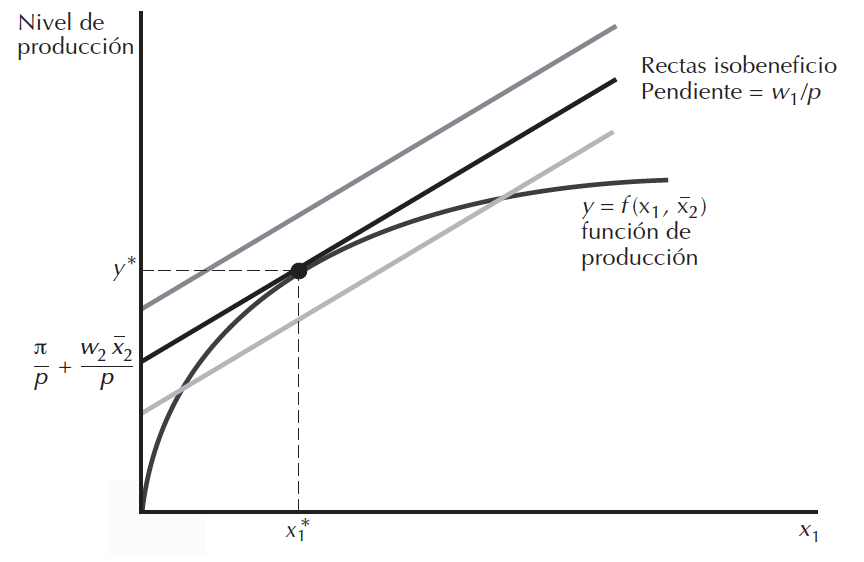
\includegraphics[width=4.5in]{figures3/maxben.png}
\end{center}
\end{frame}

\begin{frame}{\small Demandas de insumos, oferta de la firma y beneficio máximo: ¿cómo obtenerlas?}
	\begin{itemize}
		\item De la condici\'{o}n de primer orden (CPO) del problema de maximizaci\'{o}n obtendremos la \textbf{demanda no condicionada de insumo} 1 en funci\'{o}n del precio del bien final $p$ y del precio de los insumos $w_1$: $x_{1}^{*}(w_{1},p)$
		\item A partir de $x_{1}^{*}(w_{1},p)$, podremos determinar tambi\'{e}n la cantidad \'{o}ptima de producto ofrecido $y^*$. 
		
		\item La forma de obtener $y^*$ es reemplazar $x_1^*$ en la función de producci\'{o}n: $y^{*}(w_{1},p)=f(x_{1}^{*}(w_{1},p),k)$
		\item Con $y^{*}(w_{1},p)$ y $x_{1}^{*}(w_{1},p)$, tambi\'en podremos encontrar la funci\'{o}n de beneficio m\'{a}ximo de corto plazo dados los precios $(p,w_1)$: $\pi^*(w_{1},p)=py^{*}(w_{1},p)-w_{1}x_{1}^{*}(w_{1},p)-w_{2}k$
	\end{itemize}
	
\end{frame}	


%\begin{frame}{Rendimientos a escala y maximización }
%	\begin{itemize}
	
%	\item Cuando los rendimientos marginales 
%	\item En general, tendremos bien definida la soluci\'{o}n a nuestro problema, es decir, la demanda de insumo $x_{1}^{\ast }\left( w_{1},p\right)$, ser\'{a} una funci\'{o}n de los precios que resuelva el problema de maximizaci\'{o}n de beneficios de las firmas. Sin embargo, existen caracter\'{\i}sticas de la tecnolog\'{\i}a que pueden causar que nuestro problema no se encuentre bien definido.
%\item Por ejemplo, funciones del tipo $f(x_1;k)=Ax_1^2k, \ A>0$, o $f(x_1;k)=Ax_1k, \ A>0$.
%	\end{itemize}
%\end{frame}	

\begin{frame}{Est\'atica comparativa en el corto plazo}
	\begin{itemize}
	\item \textbf{Queremos analizar c\'{o}mo cambian las variables endógenas que maximizan beneficios} $(x_1^*,x_2^*,y^*,\pi^*)$ \textbf{si cambia alg\'{u}n factor que consideramos ex\'{o}geno} $(p,w_1,w_2,k)$. 
	\end{itemize}
\begin{center}
\begin{tabular}{|c|c|c|c|}
\hline
&$x_1^*$ & $y^*$ & $\pi^*$\\[6pt] 
\hline 
$\frac{\partial}{\partial w_1}$ &\color{rosee} $\leq 0$ & \color{rosee}$\leq 0$&\color{cyan}$\leq 0$\\[6pt]
\hline
$\frac{\partial}{\partial w_2}$ &\color{gray}$= 0$&\color{gray}$= 0$&\color{cyan} $<0$\\[6pt]
\hline
$\frac{\partial}{\partial p}$&\color{rosee}$\geq 0$&\color{rosee}$\geq 0$&\color{cyan}$\geq 0$\\[6pt]
\hline
$\frac{\partial}{\partial k}$&\color{rosee} $?$&\color{rosee}$?$ &\color{gray} $?$ \\[6pt]
\hline
\end{tabular}
\end{center}
\end{frame}	



\begin{frame}{Maximización de beneficios en el largo plazo}	
 \begin{itemize}
 	\item En el largo plazo, todos los \textbf{insumos son variables}, entonces la firma puede elegir de manera \'optima la cantidad de cada insumo:
 	\begin{equation*}
 	\max_{x_{1},x_{2}}pf(x_{1},x_{2})-w_{1}x_{1}-w_{2}x_{2}
 	\end{equation*}
 	
	\item \textbf{Dependiendo de la tecnología}, resolveremos el problema de maximización de beneficios:
	\begin{enumerate}
	    \item derivando y obteniendo condiciones de primer orden
	    \item analizando caso por caso (\underline{por ejemplo:} sustitutos perfectos, complementarios perfectos)
	\end{enumerate}
 \item Ejemplo del caso 1: $f(x_1,x_2)=x_1^{1/3}x_2^{1/3}$
	 \end{itemize}
	 \end{frame}
 
	 \begin{frame}{Maximización en el largo plazo: caso 1}
  \small
	 \begin{itemize}
 	\item En este caso, las CPO son las siguientes:
 	\begin{equation*}
 	pPMg_{1}(x_{1}^*,x_{2}^*)=w_{1}
 	\end{equation*}
 	\begin{equation*}
 	pPMg_{2}(x_{1}^*,x_{2}^*)=w_{2}
 	\end{equation*}

	\item Las condiciones anteriores dan lugar al siguiente resultado:
	\begin{equation*}
	TMST(x_{1}^*,x_{2}^*)=\frac{PMg_{1}(x_{1},x_{2})}{	PMg_{2}(x_{1},x_{2})}=\frac{w_{1}}{w_{2}}
	\end{equation*}
	\item Si se eligen las \textbf{demandas no condicionadas} $(x_1^*, x_2^*)$, la tasa marginal de sustituci\'on es igual al precio relativo de los insumos $\frac{w_1}{w_2}$. 
 \item La tasa a la que la firma sustituye insumos sin cambiar la cantidad producida debe ser igual a la tasa a la que se intercambian los bienes en el mercado. 
	\item De lo contrario, podr\'ia incrementar los beneficios sustituyendo insumos.
 \item En el largo plazo no vamos a chequear la CSO. Si $f(x_1,x_2)$ tiene DRS (o CRS bajo ciertos valores de $w_1, w_2$ y $p$) entonces se están maximizando los beneficios.
\end{itemize}
\end{frame}		


\begin{frame}{Maximización del beneficio en el largo plazo: caso 2}

Veamos como resolver dos ejemplos:
\begin{center}
\begin{tabular}{c|c}
\hline
   $f(x_1,x_2)=2x_1+x_2$  &  $f(x_1,x_2)=\min \{2x_1,x_2\}$  \\
   \hline
   \color{gray} ¿Beneficios de no producir?     & \color{gray} ¿Beneficios de no producir?\\
     & \\
 \color{gray} ¿Qué pasa si $\frac{w_1}{w_2}<2$?    & \color{gray}  ¿qué cumplen $x_1^*, x_2^*$ si\\ 
\color{gray}Solamente se usa $x_1$.     & \color{gray} se quiere maximizar beneficios? \\
     & \\
  \color{gray} ¿Qué pasa si $\frac{w_1}{w_2}>2$?  & \color{gray} ¿Por qué $x_1^*, x_2^*$  \\
  \color{gray} Solamente se usa $x_2$.    &\color{gray}no dependen de $w_1$ ni $w_2$? \\
     & \\
 \color{gray} ¿Qué pasa si $\frac{w_1}{w_2}=2$?    &\color{gray} ¿Beneficios de producir? \\
\end{tabular}
   \end{center} 
   \end{frame}

   

\begin{frame}{Est\'atica comparativa en el largo plazo}\small
	\begin{itemize}[leftmargin=*]
	\item \textbf{Queremos analizar c\'{o}mo cambian las variables endógenas que maximizan beneficios} $(x_1^*,x_2^*,y^*,\pi^*)$ \textbf{si cambia alg\'{u}n factor que consideramos ex\'{o}geno} $(p,w_1,w_2)$. 
	
\begin{center}
\begin{tabular}{|c|c|c|c|c|}
\hline
&$x_1^*$ & $x_2^*$& $y^*$ & $\pi^*$\\[6pt] 
\hline 
$\frac{\partial}{\partial w_1}$ & \color{rosee} $\leq 0^{(a)}$ & \color{gray} ?&\color{rosee}$\leq 0$&\color{cyan}$\leq 0$\\[6pt]
\hline
$\frac{\partial}{\partial w_2}$ &\color{gray}$?$& \color{rosee} $\leq 0^{(b)}$&\color{rosee} $\leq 0$&\color{cyan} $\leq 0$\\[6pt]
\hline
$\frac{\partial}{\partial p}$&\color{rosee}$\geq 0$&\color{rosee}$\geq 0$& \color{rosee}$\geq 0$&\color{cyan}$\geq 0$\\[6pt]
\hline
\end{tabular}
\end{center}
\item Decimos que los insumos 1 y 2 son \textbf{sustitutos} si $\frac{\partial x_1^*}{\partial w_2}>0$ y $\frac{\partial x_2^*}{\partial w_1}>0$.

\item Decimos que los insumos 1 y 2 son \textbf{complementarios} si $\frac{\partial x_1^*}{\partial w_2}<0$ y $\frac{\partial x_2^*}{\partial w_1}<0$.
\item De (a) y (b) notamos que \textbf{los insumos $x_i^*$ son bienes ordinarios}.
  \end{itemize}

  
\end{frame}	
   



\begin{frame}{Lema de Hotelling e intuición}\small
Para ver las derivadas de la última columna usamos el \textbf{Lema de Hotelling}:
		\begin{equation*}
		\frac{\partial \pi^*}{\partial p}(p,w_{1},w_{2})=y^*(p,w_{1},w_{2}); \, \frac{\partial \pi^*}{\partial w_{i}}(p,w_{1},w_{2})=-x_{i}^*(p,w_{1},w_{2})
		\end{equation*}
    \begin{itemize}
        \item Si $w_1$ aumenta, entonces la firma querrá en el margen:
        \begin{enumerate}
            \item disminuir la cantidad de insumo $1$ que demanda.
            \item elegir acordemente cuánto comprar del insumo $2$.
            \item elegir en consecuencia cuánto producir del bien final.
        \end{enumerate}
        \item Si $p$ aumenta, entonces la firma querrá en el margen
                \begin{enumerate}
                 \item aumentar la cantidad que produce del bien final.
            \item elegir acordemente cuánto demandar de cada insumo con tal de aumentar la producción.
        \end{enumerate}
    \item En cada caso, \textbf{si partimos de una solución que maximiza los beneficios y el cambio en $w_1$ o $p$ es marginal}, entonces todos los \textbf{efectos mencionados son pequeños en comparación con el cambio original}. %(corrección 14/03)
    \end{itemize}
\end{frame}

%\begin{solucion}
\begin{frame}{Lema de Hotelling}\small
\begin{itemize}

\item \textbf{¿Cu\'al es la intuici\'{o}n detr\'{a}s del Lema de Hotelling?} \small Es decir, ¿por qu\'{e} $\frac{\partial \pi^* }{\partial p}(p,w_{1},w_{2})=y^*(p,w_{1},w_{2})$? Pensemos primero lo que sucede cuando se aumenta el precio de un bien. Primero, \textit{ceteris paribus}, con el aumento del precio del bien final, los mismos bienes se vendarán m\'{a}s caros y por lo tanto aumentar\'{a}n los beneficios. Es decir, si el precio cambia en $\Delta p$, los beneficios extra que obtiene la firma es $y^*(p,w_{1},w_{2})\Delta p$.

\vspace{12pt}

\item Tambi\'en cambia cuánto se demanda de cada insumo: cuanto mayor es el precio del bien final, más desea producir la firma. Sin embargo, estamos pensando en cambios marginales infinitesimales. En esos niveles de cambio, un cambio en la cantidad de bien final puede ser descartada. Por lo tanto, el \'{u}nico efecto que es considerable es $y(p,w_{1},w_{2})\Delta p$, entonces: $\Delta \pi ^{\ast}=y^*(p,w_{1},w_{2})\Delta p$, que, reordenando y tomando $\Delta\rightarrow 0$, tenemos: $\frac{\partial \pi ^{\ast }}{\partial p}=y^*(p,w_{1},w_{2})$.
\end{itemize}
\end{frame}
%\end{solucion}



\begin{frame}{\small Propiedades de $y^*(w_1, w_2,p)$, $x_i^*(w_1, w_2,p)$ y $\pi^* (p,w_{1},w_{2})$}	
Para una \textbf{tecnología monótona}, las funciones de oferta $y(p,\textbf{w})$ y de beneficio $\pi(p,\textbf{w})$ satisfacen las siguientes
propiedades:
\begin{itemize}
\item \color{cyan} Las funciones de oferta y demanda de insumos son homog\'{e}neas de grado 0. \color{black}\textbf{Esto nos dice que las cantidades utilizadas de insumos y de producto producido dependen solamente de los precios relativos y no del nivel general de precios.} $\forall t>0$:
\begin{center}
$\hspace{-3em}x_{i}^*(tp,tw_{1},tw_{2})=x_{i}^*(p,w_{1},w_{2}); \, y^*(tp,tw_{1},tw_{2})=y^*(p,w_{1},w_{2})$
\end{center}
\item \color{rosee}Dado que las funciones de demanda y oferta son homog\'{e}neas de grado
0, obtenemos que la funci\'{o}n de beneficio m\'{a}ximo es homog\'{e}nea de grado 1. \color{black} $\forall t>0$: 
\begin{center}
$\pi^* (tp,tw_{1},tw_{2})=t\pi^* (p,w_{1},w_{2})$
\end{center}

\end{itemize}
\end{frame}

\begin{frame}{ Beneficios de LP \textbf{en equilibrio} si $f(x_1,x_2)$ tiene CRS}

\color{cyan}\textbf{Proposición:} \color{black} Sea $f(x_1,x_2)$ con rendimientos constantes a escala (CRS). Entonces, si el problema de maximización de beneficios tiene soluci\'on, los beneficios de largo plazo (LP) \textbf{en equilibrio} son iguales a cero.

\textit{Este resultado es razonable en algunos contextos, por ejemplo existe libre entrada de firmas en la industria. }
\medskip

\color{cyan}\textbf{Demostración:} \color{black} Si $f\left( x_1,x_2\right) $ tiene CRS, vale que  \[\color{rosee}f(tx_1,tx_2)=tf(x_1,x_2)\color{black}, \text{ para cualesquiera } t>1; (x_1,x_2)\in \mathbb{R}_{+}^2.\] 
Tomando $t=2$ y $(0,0)$ notamos que vale que $f(0,0)=0$.  Por lo tanto, si la firma utilizara $(x_1,x_2)=(0,0)$ la firma puede obtener beneficios iguales a cero. Por lo tanto, el beneficio máximo $\pi^*$ es mayor (o igual) al beneficio de producir usando $(0,0)$ de los insumos. 
\begin{center}
$\pi ^{\ast }\geq 0 \qquad (A)$
\end{center}

\end{frame}

\begin{frame}{ Beneficios de LP \textbf{en equilibrio} si $f(x_1,x_2)$ tiene CRS}

Veamos ahora que, \textbf{en equilibrio},\footnote{Es decir, solamente para el caso donde la firma quiere producir cantidades positivas y finitas.} el beneficio máximo es igual a cero.  Llamemos $(x_1^*, x_2^*)$ a las cantidades de insumos que maximizan beneficios, entonces: 
\begin{center}
$\pi ^{\ast }=\pi(x_1^{\ast },x_2^{\ast })=pf(x_1^{\ast },x_2^{\ast })-w_1x_1^{\ast }+w_2x_2^{\ast }$. 
\end{center}

Eligiendo otras cantidades de insumos, $(tx_1^*,tx_2^{\ast })$ (\textbf{con} $t>1$): \begin{align*}
    \pi(x_1^{\ast },x_2^{\ast }) \geq &\pi(tx_1^{\ast },tx_2^{\ast })=p\color{rosee}f(tx_1^{\ast },tx_2^{\ast })\color{black}-w_1tx_1^{\ast }+w_2tx_2^{\ast }\\
    &\geq p\color{rosee}tf(x_1^{\ast },x_2^{\ast })\color{black}-w_1tx_1^{\ast }+w_2tx_2^{\ast }\\
    &\geq t( p\color{rosee}f(x_1^{\ast },x_2^{\ast })\color{black}-w_1x_1^{\ast }+w_2x_2^{\ast })=t\pi(x_1^*,x_2^*)\end{align*}

Entonces  $(1-t)\pi^* \geq 0 \qquad (B)$, donde $t>1$.

Por $(A)$ y por $(B)$ se tiene que $\pi^*=0$.
%Dado que este es el beneficio m\'{a}ximo, $\forall \textbf{x}' \neq \textbf{x}^{\ast }:$
%\begin{center}
%$\pi ^{\ast }\geq pf(\textbf{x}')-\sum\limits_{i=1}^{n}w_{i}x_{i}'$
%\end{center}
%En particular, esto tiene que ser cierto para $\textbf{x}'=t\textbf{x}^{\ast},$ con $t>1:$
%\begin{center}
%$\pi^{\ast }\geq pf(t\textbf{x}^{\ast })-\sum\limits_{i=1}^{n}w_{i}tx_{i}^{\ast }=t\pi
%^{\ast }$
%\end{center}
%Es decir que $\pi ^{\ast }(t-1)\leq 0$ o $\pi ^{\ast }\leq 0.$ Por lo tanto, si $\pi^*\geq 0$ y $\pi^*\leq 0$ se tiene que $\pi^*=0$.\qed 

\end{frame}

\begin{frame}{Ejercicio $2.14^B$ - Ejercicio para practicar}
    Suponga una firma que produce un bien final empleando un único insumo ($x$). Su tecnología de producción viene dada por la siguiente función de producción
\begin{equation*}
    q = f(x) = \begin{cases}
    2x & \text{  si  } x \leq 1 \\
    x + 1 & \text{  si  } x > 1
    \end{cases}
\end{equation*}
El precio del bien final es $p=1$ y el precio del insumo es $w>0$.

\begin{enumerate}[label=(\alph*)]
    \item Grafique el conjunto de producción. ¿Es este conjunto convexo? Justifique su respuesta.
    \item Suponga que $w=3/2$. Formule el problema de maximización de beneficios y encuentre la cantidad de insumo contratada y la cantidad producida. 
    \item ¿Cómo se modifica su respuesta del punto (b) si $w=2$?
    \item ¿Cómo se modifica su respuesta del punto (b) si $w=1$?
    \item ¿Para qué valores de $w$ es óptimo para la firma no producir? Explique intuitivamente el resultado.
\end{enumerate}
\end{frame}

\begin{frame}[noframenumbering]{}
   \begin{center}
       \Large Ap\'endice - el contenido de las siguientes slides es optativo
   \end{center} 
\end{frame}

\begin{frame}[noframenumbering]{Est\'atica comparativa en el corto plazo}
	\begin{itemize}
		\item Si la funci\'{o}n de producci\'{o}n es \textbf{estrictamente c\'{o}ncava}\footnote{Recordemos que cuando decimos que una función es cóncava también admitimos el caso donde $f$ sea lineal.}, entonces la soluci\'{o}n
del problema de maximizaci\'{o}n de beneficios es $x_{1}^*(p,w_{1},w_{2},k)$
tal que:
\begin{center}
$pPMg_{1}(x_{1}^*(p,w_{1},w_{2},k),k)=w_{1} \quad (*)$ 
\end{center}
\item Derivamos $(*)$ respecto de $p$, $w_1$, $w_2$ y $k$.
		\item Si se da un cambio en $p$:
		\begin{equation*}
	\color{red}	\underbrace{PMg_{1}(x_{1}^{*}(\cdot))}_{>0}\color{black}+p\color{blue}\underbrace{\frac{\partial PMg_{1}}{\partial{x_{1}}}(x_{1}^{*}(\cdot))}_{<0}\color{black}\frac{\partial x_{1}}{\partial p}(\cdot)=0
		\end{equation*}
		\item Dado que la productividad marginal es \color{red}positiva \color{black}y \color{blue}decreciente\color{black}, y $p>0$, debe
ser que $\frac{\partial x_{1}}{\partial p}(w_{1},p,w_{2},k)>0$.
	\end{itemize}
\end{frame}	

\begin{frame}[noframenumbering]{Est\'atica comparativa en el corto plazo} \small
	\begin{itemize}
		\item Ante cambio en $w_{1}$:
		\begin{equation*}
		p\color{blue}\underbrace{\frac{\partial{PMg_{1}}}{\partial{x_{1}}}(x_{1}^{*}(w_{1},p,w_{2},k),k)}_{<0}\color{black}\frac{\partial x_{1}}{\partial w_{1}}(w_{1},p,w_{2},k)=1
		\end{equation*}
		\item Lo cual implica que:
		\begin{equation*}
		\frac{\partial x_{1}}{\partial w_{1}}(w_{1},p,w_{2},k)<0
		\end{equation*}
	\end{itemize}
\end{frame}
\begin{frame}[noframenumbering]{Est\'atica comparativa en el corto plazo}
	\begin{center}
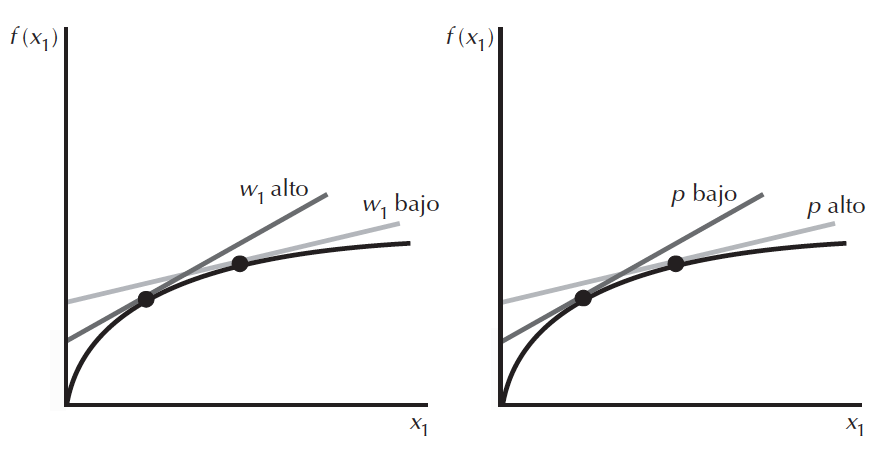
\includegraphics[width=4.5in]{figures3/static.png}
\end{center}
\end{frame}

\begin{frame}[noframenumbering]{Est\'atica comparativa en el corto plazo} \small

	\begin{itemize}
	\item Supongamos ahora que var\'{\i}a el precio del insumo 2, $w_{2}$:
\[
p\frac{\partial PMg_{1}}{\partial x_{1}}(x_{1}^*(p,w_{1},w_{2},k),k)\frac{\partial x_{1}}{\partial w_{2}}(p,w_{1},w_{2},k)=0
\]
lo cual implica que:
\[
\frac{\partial x_{1}}{\partial w_{2}}(p,w_{1},w_{2},k)=0
\]
\item En efecto, en este contexto en el que el insumo 2 est\'{a} fijo, un cambio
en $w_{2}$ es un cambio en los costos fijos, que no afectan las decisiones
de producci\'{o}n.
	\end{itemize}
\end{frame}		

\begin{frame}[noframenumbering]{Est\'atica comparativa en el corto plazo} \small
	\begin{itemize}
\item Por \'{u}ltimo, si $k$ aumenta, se puede combinar los insumos de maneras que antes no eran posibles:

\[
p\left(\frac{\partial PMg_{1}}{\partial x_{1}}(x_{1}^*(\cdot))\frac{\partial x_{1}}{\partial k}(p,w_{1},w_{2},k)+\frac{\partial PMg_{1}}{\partial x_{2}}(x_{1}^*(\cdot))\right)=0
\]
\item El signo de $\frac{\partial x_{1}}{\partial k}(p,w_{1},w_{2},k)$ depender\'{a}, entonces de c\'{o}mo var\'{\i}a la productividad marginal del insumo 1 cuando aumenta la cantidad de insumo 2. En todos los casos,
\[
\frac{\partial y}{\partial a}(p,w_{1},w_{2},k)=PMg_{1}(x_{1}(p,w_{1},w_{2},k),k)\frac{\partial x_1}{\partial a}
\]
para $a = p, w_{1}, w_{2}, k$.
\item Por lo tanto, el signo del cambio en la oferta es id\'{e}ntico al signo del cambio en la demanda del insumo 1.
	\end{itemize}
	\end{frame}

 \begin{frame}[noframenumbering]{Lema de Hotelling derivando respecto de $w_1$}\small
\[\frac{\partial \pi^*}{\partial w_{i}}(p,w_{1},w_{2})=-x_{i}^*(p,w_{1},w_{2})\]
\begin{proof}
La funci\'{o}n de beneficio m\'{a}ximo es: 
\begin{center}
$\pi ^{\ast
}(p,\textbf{w})=pf^{\ast }\left( x_{1}^{\ast }(p,\textbf{w}),x_{2}^{\ast
}(p,\textbf{w})\right)-w_{1}x_{1}^{\ast }(p,\textbf{w})-w_{2}x_{2}^{\ast
}(p,\textbf{w})$. 
\end{center}
Diferenciando la misma con respecto a $w_{1}$:

\begin{eqnarray*}
\frac{\partial \pi ^{\ast }}{\partial w_{1}} &=&p\frac{\partial y^{\ast }}{%
\partial x_{1}}\frac{\partial x_{1}^{\ast }}{\partial w_{1}}+p\frac{\partial
y^{\ast }}{\partial x_{2}}\frac{\partial x_{2}^{\ast }}{\partial w_{1}}-w_{1}%
\frac{\partial x_{1}^{\ast }}{\partial w_{1}}-x_{1}^{\ast
}(p,w_{1},w_{2})-w_{2}\frac{\partial x_{2}^{\ast }}{\partial w_{1}} \\
&=&\underset{=0 \ por \ CPO}{\underbrace{\left[ p\frac{\partial y^{\ast }}{\partial x_{1}%
}-w_{1}\right] }}\frac{\partial x_{1}^{\ast }}{\partial w_{1}}-\underset{=0 \ por \ CPO}{%
\underbrace{\left[ p\frac{\partial y^{\ast }}{\partial x_{2}}-w_{2}\right] }}\frac{\partial x_{2}^{\ast }}{\partial w_{1}}%
-x_{1}^{\ast } \\
&=&-x_{1}^{\ast }(p,w_{1},w_{2})
\end{eqnarray*}
\end{proof}
\end{frame}

\begin{frame}[noframenumbering]{Lema de Hotelling derivando respecto de $p$}\small
\[\frac{\partial \pi^*}{\partial p}(p,w_{1},w_{2})=y^*(p,w_{1},w_{2})\]
\begin{proof}
La funci\'{o}n de beneficio m\'{a}ximo es: 
\begin{center}
$\pi ^{\ast
}(p,\textbf{w})=pf^{\ast }\left( x_{1}^{\ast }(p,\textbf{w}),x_{2}^{\ast
}(p,\textbf{w})\right)-w_{1}x_{1}^{\ast }(p,\textbf{w})-w_{2}x_{2}^{\ast
}(p,\textbf{w})$. 
\end{center}
Diferenciando la misma con respecto a $p$:

\begin{eqnarray*}
\frac{\partial \pi ^{\ast }}{\partial p} &=& y^* +p\frac{\partial y^{\ast }}{%
\partial x_{1}}\frac{\partial x_{1}^{\ast }}{\partial p}+p\frac{\partial
y^{\ast }}{\partial x_{2}}\frac{\partial x_{2}^{\ast }}{\partial p}-w_{1}%
\frac{\partial x_{1}^{\ast }}{\partial p}-w_{2}\frac{\partial x_{2}^{\ast }}{\partial p} \\
&=&\underset{=0 \ por \ CPO}{\underbrace{\left[ p\frac{\partial y^{\ast }}{\partial x_{1}%
}-w_{1}\right] }}\frac{\partial x_{1}^{\ast }}{\partial p}-\underset{=0 \ por \ CPO}{%
\underbrace{\left[ p\frac{\partial y^{\ast }}{\partial x_{2}}-w_{2}\right] }}\frac{\partial x_{2}^{\ast }}{\partial p}%
-x_{1}^{\ast } \\
&=&y^{\ast }(p,w_{1},w_{2})
\end{eqnarray*}
\end{proof}
\end{frame}

\end{document}